\documentclass{standalone}
\usepackage{tikz}
\usetikzlibrary{patterns, positioning}


\begin{document}
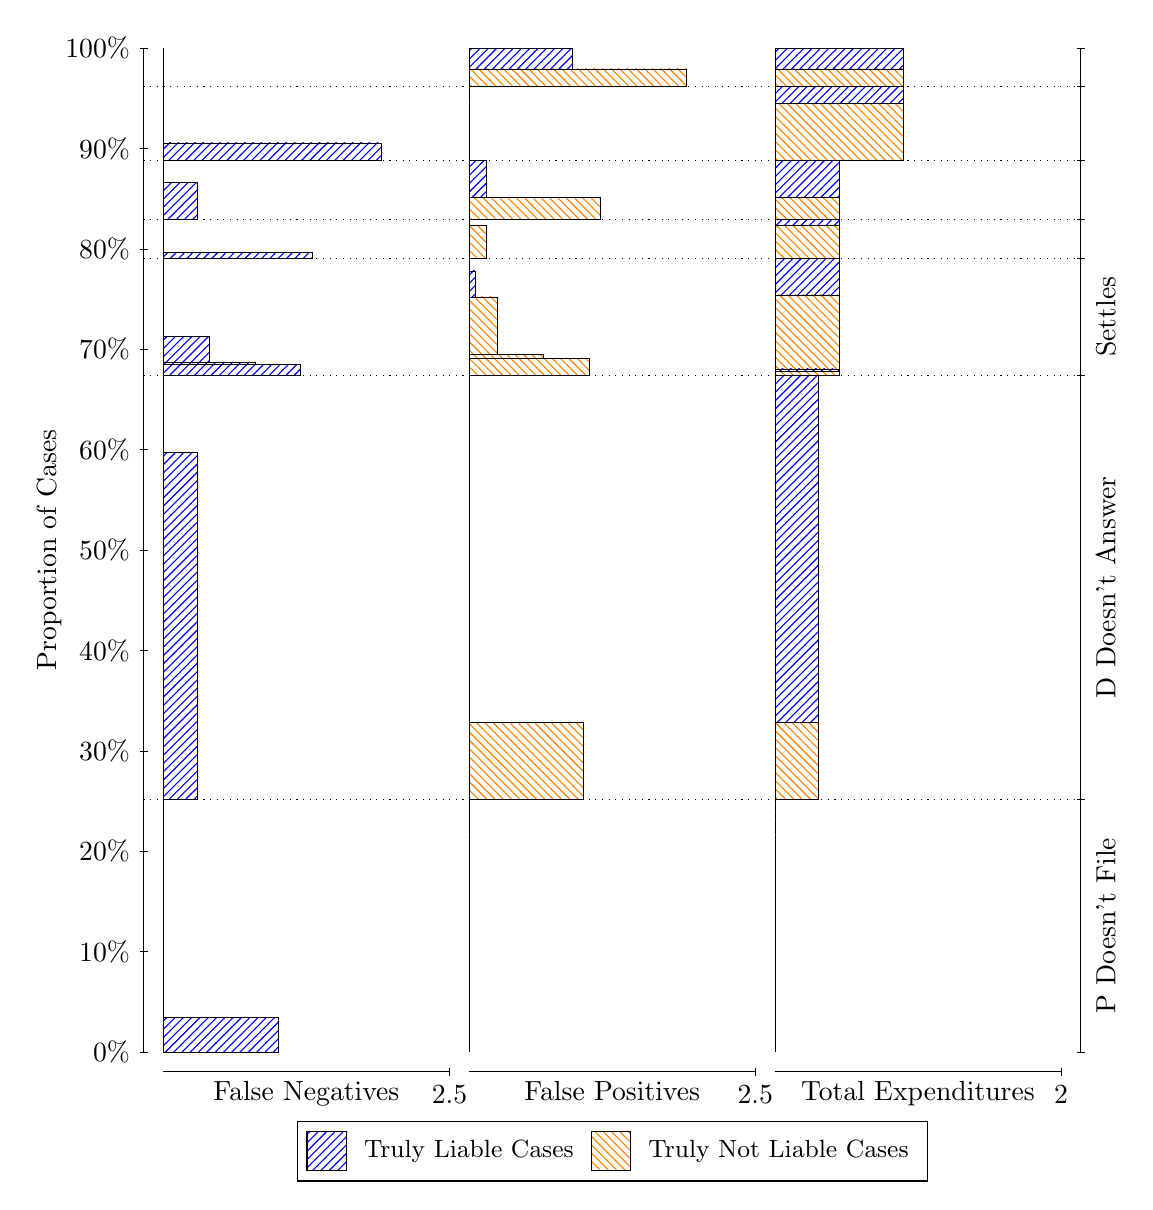
\begin{tikzpicture}
\draw[black, very thin] (1.5,1.75) -- (1.5,14.5);
\node[rotate=90, text=black, anchor=center] at (0.3, 8.125) {Proportion of Cases};
\draw[black, very thin] (1.45,1.75) -- (1.55,1.75);
\node[text=black, anchor=east] at (1.45, 1.75) {0\%};
\draw[black, very thin] (1.45,3.025) -- (1.55,3.025);
\node[text=black, anchor=east] at (1.45, 3.025) {10\%};
\draw[black, very thin] (1.45,4.3) -- (1.55,4.3);
\node[text=black, anchor=east] at (1.45, 4.3) {20\%};
\draw[black, very thin] (1.45,5.575) -- (1.55,5.575);
\node[text=black, anchor=east] at (1.45, 5.575) {30\%};
\draw[black, very thin] (1.45,6.85) -- (1.55,6.85);
\node[text=black, anchor=east] at (1.45, 6.85) {40\%};
\draw[black, very thin] (1.45,8.125) -- (1.55,8.125);
\node[text=black, anchor=east] at (1.45, 8.125) {50\%};
\draw[black, very thin] (1.45,9.4) -- (1.55,9.4);
\node[text=black, anchor=east] at (1.45, 9.4) {60\%};
\draw[black, very thin] (1.45,10.675) -- (1.55,10.675);
\node[text=black, anchor=east] at (1.45, 10.675) {70\%};
\draw[black, very thin] (1.45,11.95) -- (1.55,11.95);
\node[text=black, anchor=east] at (1.45, 11.95) {80\%};
\draw[black, very thin] (1.45,13.225) -- (1.55,13.225);
\node[text=black, anchor=east] at (1.45, 13.225) {90\%};
\draw[black, very thin] (1.45,14.5) -- (1.55,14.5);
\node[text=black, anchor=east] at (1.45, 14.5) {100\%};

\draw[black, very thin] (13.4,1.75) -- (13.4,14.5);
\draw[black, very thin] (13.35,1.75) -- (13.45,1.75);
\node[anchor=west] at (13.35, 1.75) {};
\draw[black, very thin] (13.35,4.9538) -- (13.45,4.9538);
\node[anchor=west] at (13.35, 4.9538) {};
\draw[black, very thin] (13.35,10.346) -- (13.45,10.346);
\node[anchor=west] at (13.35, 10.346) {};
\draw[black, very thin] (13.35,11.832) -- (13.45,11.832);
\node[anchor=west] at (13.35, 11.832) {};
\draw[black, very thin] (13.35,12.321) -- (13.45,12.321);
\node[anchor=west] at (13.35, 12.321) {};
\draw[black, very thin] (13.35,13.072) -- (13.45,13.072);
\node[anchor=west] at (13.35, 13.072) {};
\draw[black, very thin] (13.35,14.016) -- (13.45,14.016);
\node[anchor=west] at (13.35, 14.016) {};
\draw[black, very thin] (13.35,14.5) -- (13.45,14.5);
\node[anchor=west] at (13.35, 14.5) {};

\draw[black, very thin, pattern color=blue, pattern=north east lines] (1.75,1.75) rectangle (3.2033,2.1914);
\draw[black, very thin, pattern color=orange, pattern=north west lines] (1.75,2.1914) rectangle (1.75,4.9538);
\draw[black, very thin, pattern color=blue, pattern=north east lines] (1.75,4.9538) rectangle (2.186,9.3674);
\draw[black, very thin, pattern color=orange, pattern=north west lines] (1.75,9.3674) rectangle (1.75,10.346);
\draw[black, very thin, pattern color=blue, pattern=north east lines] (1.75,10.346) rectangle (3.494,10.485);
\draw[black, very thin, pattern color=blue, pattern=north east lines] (1.75,10.485) rectangle (2.9127,10.509);
\draw[black, very thin, pattern color=blue, pattern=north east lines] (1.75,10.509) rectangle (2.3313,10.839);
\draw[black, very thin, pattern color=orange, pattern=north west lines] (1.75,10.839) rectangle (1.75,11.832);
\draw[black, very thin, pattern color=blue, pattern=north east lines] (1.75,11.832) rectangle (3.6393,11.905);
\draw[black, very thin, pattern color=orange, pattern=north west lines] (1.75,11.905) rectangle (1.75,12.321);
\draw[black, very thin, pattern color=blue, pattern=north east lines] (1.75,12.321) rectangle (2.186,12.79);
\draw[black, very thin, pattern color=orange, pattern=north west lines] (1.75,12.79) rectangle (1.75,13.072);
\draw[black, very thin, pattern color=blue, pattern=north east lines] (1.75,13.072) rectangle (4.5113,13.294);
\draw[black, very thin, pattern color=orange, pattern=north west lines] (1.75,13.294) rectangle (1.75,14.016);
\draw[black, very thin, pattern color=orange, pattern=north west lines] (1.75,14.016) rectangle (1.75,14.236);
\draw[black, very thin, pattern color=blue, pattern=north east lines] (1.75,14.236) rectangle (1.75,14.5);
\draw[black, very thin, pattern color=orange, pattern=north west lines] (5.6333,1.75) rectangle (5.6333,4.5123);
\draw[black, very thin, pattern color=blue, pattern=north east lines] (5.6333,4.5123) rectangle (5.6333,4.9538);
\draw[black, very thin, pattern color=orange, pattern=north west lines] (5.6333,4.9538) rectangle (7.0867,5.9328);
\draw[black, very thin, pattern color=blue, pattern=north east lines] (5.6333,5.9328) rectangle (5.6333,10.346);
\draw[black, very thin, pattern color=orange, pattern=north west lines] (5.6333,10.346) rectangle (7.1593,10.556);
\draw[black, very thin, pattern color=orange, pattern=north west lines] (5.6333,10.556) rectangle (6.578,10.609);
\draw[black, very thin, pattern color=orange, pattern=north west lines] (5.6333,10.609) rectangle (5.9967,11.34);
\draw[black, very thin, pattern color=blue, pattern=north east lines] (5.6333,11.34) rectangle (5.706,11.67);
\draw[black, very thin, pattern color=blue, pattern=north east lines] (5.6333,11.67) rectangle (5.6333,11.832);
\draw[black, very thin, pattern color=orange, pattern=north west lines] (5.6333,11.832) rectangle (5.8513,12.248);
\draw[black, very thin, pattern color=blue, pattern=north east lines] (5.6333,12.248) rectangle (5.6333,12.321);
\draw[black, very thin, pattern color=orange, pattern=north west lines] (5.6333,12.321) rectangle (7.3047,12.603);
\draw[black, very thin, pattern color=blue, pattern=north east lines] (5.6333,12.603) rectangle (5.8513,13.072);
\draw[black, very thin, pattern color=orange, pattern=north west lines] (5.6333,13.072) rectangle (5.6333,13.794);
\draw[black, very thin, pattern color=blue, pattern=north east lines] (5.6333,13.794) rectangle (5.6333,14.016);
\draw[black, very thin, pattern color=orange, pattern=north west lines] (5.6333,14.016) rectangle (8.3947,14.236);
\draw[black, very thin, pattern color=blue, pattern=north east lines] (5.6333,14.236) rectangle (6.9413,14.5);
\draw[black, very thin, pattern color=orange, pattern=north west lines] (9.5167,1.75) rectangle (9.5167,4.5123);
\draw[black, very thin, pattern color=blue, pattern=north east lines] (9.5167,4.5123) rectangle (9.5167,4.9538);
\draw[black, very thin, pattern color=orange, pattern=north west lines] (9.5167,4.9538) rectangle (10.062,5.9328);
\draw[black, very thin, pattern color=blue, pattern=north east lines] (9.5167,5.9328) rectangle (10.062,10.346);
\draw[black, very thin, pattern color=orange, pattern=north west lines] (9.5167,10.346) rectangle (10.334,10.399);
\draw[black, very thin, pattern color=blue, pattern=north east lines] (9.5167,10.399) rectangle (10.334,10.424);
\draw[black, very thin, pattern color=orange, pattern=north west lines] (9.5167,10.424) rectangle (10.334,11.364);
\draw[black, very thin, pattern color=blue, pattern=north east lines] (9.5167,11.364) rectangle (10.334,11.832);
\draw[black, very thin, pattern color=orange, pattern=north west lines] (9.5167,11.832) rectangle (10.334,12.248);
\draw[black, very thin, pattern color=blue, pattern=north east lines] (9.5167,12.248) rectangle (10.334,12.321);
\draw[black, very thin, pattern color=orange, pattern=north west lines] (9.5167,12.321) rectangle (10.334,12.603);
\draw[black, very thin, pattern color=blue, pattern=north east lines] (9.5167,12.603) rectangle (10.334,13.072);
\draw[black, very thin, pattern color=orange, pattern=north west lines] (9.5167,13.072) rectangle (11.152,13.794);
\draw[black, very thin, pattern color=blue, pattern=north east lines] (9.5167,13.794) rectangle (11.152,14.016);
\draw[black, very thin, pattern color=orange, pattern=north west lines] (9.5167,14.016) rectangle (11.152,14.236);
\draw[black, very thin, pattern color=blue, pattern=north east lines] (9.5167,14.236) rectangle (11.152,14.5);
\draw[black, dotted] (1.5,4.9538) -- (13.4,4.9538);
\draw[black, dotted] (1.5,10.346) -- (13.4,10.346);
\draw[black, dotted] (1.5,11.832) -- (13.4,11.832);
\draw[black, dotted] (1.5,12.321) -- (13.4,12.321);
\draw[black, dotted] (1.5,13.072) -- (13.4,13.072);
\draw[black, dotted] (1.5,14.016) -- (13.4,14.016);
\draw[black, very thin] (1.75,1.5) -- (5.3833,1.5);
\node[text=black, anchor=north] at (3.5667, 1.5) {False Negatives};
\draw[black, very thin] (5.3833,1.45) -- (5.3833,1.55);
\node[text=black, anchor=north] at (5.3833, 1.45) {2.5};

\draw[black, very thin] (5.6333,1.5) -- (9.2667,1.5);
\node[text=black, anchor=north] at (7.45, 1.5) {False Positives};
\draw[black, very thin] (9.2667,1.45) -- (9.2667,1.55);
\node[text=black, anchor=north] at (9.2667, 1.45) {2.5};

\draw[black, very thin] (9.5167,1.5) -- (13.15,1.5);
\node[text=black, anchor=north] at (11.333, 1.5) {Total Expenditures};
\draw[black, very thin] (13.15,1.45) -- (13.15,1.55);
\node[text=black, anchor=north] at (13.15, 1.45) {2};

\node[text=black, centered, rotate=90] at (13.72, 3.3519) {P Doesn't File};
\node[text=black, centered, rotate=90] at (13.72, 7.6501) {D Doesn't Answer};
\node[text=black, centered, rotate=90] at (13.72, 11.089) {Settles};





\draw (7.449999999999999,1.5) node[draw=none] (baseCoordinate) {};
\begin{scope}[align=center]
        \matrix[scale=0.5, draw=black, below=0.5cm of baseCoordinate, nodes={draw}, column sep=0.1cm]{
            \node[rectangle, draw, minimum width=0.5cm, minimum height=0.5cm, pattern color=blue, pattern=north east lines] {}; &
            \node[draw=none, font=\small, text=black] (B) {Truly Liable Cases}; &
            \node[rectangle, draw, minimum width=0.5cm, minimum height=0.5cm, pattern color=orange, pattern=north west lines] {}; &
            \node[draw=none, font=\small, text=black] (B) {Truly Not Liable Cases}; \\
            };
\end{scope}

\end{tikzpicture}
\end{document}